\documentclass[a4paper, 11pt]{article}
\usepackage{graphicx}
\usepackage{pdflscape}
\usepackage{titlesec}

\setcounter{secnumdepth}{4}

\usepackage[left=2cm, text={17cm, 24cm}, top= 3cm]{geometry}
\usepackage[utf8]{inputenc}
\usepackage[czech]{babel}
\title{IDS}
\author{Petr Kaška}
\date{February 2023}

\begin{document}
 
    \begin{titlepage}
        
        \begin{center}
        
            {\Huge\textsc{ Vysoké učení technické v Brně\\
            \huge Fakulta informačních technologií}\\}
            
             \vspace{\stretch{0.382}}
             
             {\LARGE \Huge{1.~Část projektu IDS\\ }}
             
                \vspace{0.5cm}
                
             {\LARGE zadání IUS 37. Rezervace letenek}
               \vspace{\stretch{0.618}}
            
           \end{center} 
            
            {\LARGE 
            {Petr Kaška (xkaska01)\\
            Martin Hemza (xhemza05)}}
            
    \end{titlepage}
    \section{Zadání:}
    \Large{Vaším úkolem je navrhnout webovou aplikaci pro rezervaci letenek. Systém musí uživateli umožnit specifikovat požadavek pomocí místa odletu a příletu, data, času, třídy, letecké společnosti apod. Jedno letadlo může létat na více letech, stejně tak mezi dvěmi destinacemi může létat více letadel různých společností. Zákazník si rezervuje letenku, která může být na několik letů, i různých společností (např. letenka Praha  $\rightarrow$ San Francisco s lety Praha $\rightarrow$ Londýn ČSA, Londýn  $\rightarrow$ San Francisco British Airways). Systém musí umožnit klientovi tisk letového itineráře, který obsahuje informace o dobách příletů a odletů na jednotlivých letištích. Každý typ letadla má různý počet sedadel a jejich rozvržení do tříd. Nemodelujte jednotlivá sedadla. Rezervací může klient zamluvit i více míst v jednom letu. Technická mezipřistání modelovat nemusíte. Systém musí evidovat, která společnost kdy, odkud a kam létá. Cena sedadla v dané třídě může být u každé společnosti jiná, cena letenky je dána součtem cen všech rezervovaných sedadel na všech letech. Pokud klient rezervovanou letenku včas nezaplatí, rezervace se z databáze smaže.}

    \section{Popis ERD:}
        \large{       Tento systém rezervace letenek je rozdělen do devíti entitních množin, jedné generalizace/specializace a třemi vazebními vztahy. Existují dva druhy uživatelů: zákazník a cestovní agent. Pro cestovního agenta jsou k dispozici některé atributy, které zákazník nemá, a proto jsme použili generalizaci/specializaci pro cestovního agenta a zákazníka.

Systém obsahuje silnou entitu "lístek", kde každý zákazník může koupit více lístků, ale každý konkrétní lístek je vždy pro jednoho zákazníka. Toto jsme modelovali pomocí vztahu 1:N. Dále je k dispozici silná entitní množina "třída", vazební množina "rozložení sedadel" a silná entitní množina "letadlo", kde instance právě jedné třídy a právě jednoho letadla musí vždy mít stejný počet sedadel. Dále jsme navrhli silnou entitní množinu "aerolinka", protože aerolinky obvykle mají více letadel a víc letů, takže jsme použili vztahy 1:N. Další silnou entitní množinou jsou "let" a "trať". Trasy se obvykle často nemění a létá po nich více letadel různých aerolinií, proto jsme to namodelovali tímto způsobem. Vazební množina "cena třídy" udává cenu jednotlivých lístků v různých třídách jednoho letu.

Následně jsme modelovali Množinu Letový plán, díky které jsme schopni zaznamenat časy přistání a odletů jednotlivých letů.
        
        \section{Popis Use Case:}
         \large{Systém se skládá ze 3 aktérů zákazníka, cestovního agenta a administrátora. U zákazníka jsme použili include. Abychom zdůraznily změnu stav letenky na koupená/rezervovaná při interakci s nimi.}
        
  
    \begin{landscape}
    
        
\includegraphics[scale=0.8]{ERD.png}

    \end{landscape}
   
    
\includegraphics[scale=0.85]{USECASE.png}
    \newpage

    \section{SQL skript pro vytvoření pokročilých objektů schématu databáze}
    \subsection{Triggery}
    \subsubsection{dolar\_convertor}
        Trigger, ktery slouzi k prevadeni ceny jednotlivych trid z korun na dolary, spousti se pri vlozeni nove tridy
    \subsubsection{date\_of\_birth\_check}
        Trigger,  ktery zkontroluje zda jsou data narozeni jednotlivych klientu spravna (dny v jednotlivych mesicich, prestupny rok, ...). Spousti se pri vlozeni zakaznikova data narozeni  
    \subsubsection{update\_seats\_available}
        Trigger slouží k aktualizaci počtu dostupných sedadel v tabulce \textbf{SEAT\_CONFIGURATION} na základě počtu rezervovaných sedadel v tabulce \textbf{RESERVATION}. Pokud se jedná o operaci vkládání nebo aktualizace, počet rezervovaných sedadel se získá z řádku \textbf{NEW}. Pokud jde o operaci mazání, počet rezervovaných sedadel se získá jako opačná hodnota počtu sedadel v řádku \textbf{NEW}. Poté je provedena aktualizace počtu sedadel v tabulce \textbf{SEAT\_CONFIGURATION}. Řádek s odpovídajícím \textbf{AIRPLANE\_ID} je vyhledán pomocí poddotazu, který získává hodnotu \textbf{AITPLANE\_ID} z tabulky \textbf{FLIGHT\_SCHEDULE} na základě hodnoty \textbf{FLIGHT\_SCHEDULE\_ID} z řádku \textbf{NEW}. Aktualizace je provedena pouze pro řádky, kde \textbf{CLASS\_ID} odpovídá hodnotě \textbf{CLASS\_ID} z řádku \textbf{NEW}.
     \subsection{Procedury}
        \subsubsection{show\_customers\_on\_route}
        procedura, ktery vypise jmena klientu, kteri maji listek na prislusne trase show\_customers\_on\_route (odletova destinace, priletova destinace)
    \subsubsection{print\_customer\_names}
     procedura, ktera vypise vsechna jmena zakazniku, kteri jsou momentalne v databazi
    \subsection{Explain plan}
        Explain plan nám umožňuje zjistit postupnost a počet kroků, které se použijí při přístupu k udájům v systému relačních databází. V našem skriptu jsme zjistili posloupnost kroků pro dotaz \textbf{Kolik průměrně utratil zakaznik s id 2 za letenky}. Následně jsme vykonali optimalizaci pomocí vytvoření indexu pro sloupec \textbf{ID\_uživatele} z tabulky \textbf{Ticket} a index pro sloupec, který v tabulce  \textbf{Class\_price} uchovává id jednotlivých tříd \textbf{id\_třídy}. Díky přístupu přímo k indexům se vyhledávání urychlilo, protože nebylo v daných případech nutné přistupovat k celé tabulce. Uspěšnou optimalizaci jsme ověřili opětovným použitím  příkazu po optimalizaci na stejný dotaz

    \subsection{Přístupová práva}
    Přístupová práva pro druhého člena týmu jsme vyřešili pomocí \textbf{GRANT ALL} pro všechny tabulky definované v naší databázi, procedury a materializovaný pohled.Tím pádem je druhý uživatel taktéž administrátor, protože má plný přístup

    \subsection{Materializovaný pohled}
    Vytvořili jsme materializovaný pohled s názvem \textbf{Agent\_view}, který obsahuje sloupce \textbf{first\_name}, \textbf{last\_name} a \textbf{commision} ze dvou tabulek \textbf{Travel\_Agent} a \textbf{Customer}. Pohled bude automaticky obnovován po každé provedené transakci. Následující Select vypisuje obsah materializovaného pohledu.
    Poté provedeme UPDATE, který aktualizuje hodnotu \textbf{commision} agenta s id 1 v tabulce \textbf{Travel\_Agent}.
    
    \subsection{Transakce}
     \subsubsection{tran. 1}
 tato transakce vlozi noveho zakaznika "Johna Doe" a pote vytvori jeho listek se statusem "unbooked", vytvori mu 1 rezervaci do ekonomicke tridy a ticket status nastavi na booked. Atomicnost - BEGIN(zajistit provadeni kodu jako celku), COMMIT(dokonci transakci) a ROLLBACK(v pripade nedokonceni transakce vrati zpet zmeny a udrzi konzistenci databaze)

     \subsubsection{tran. 2}
    Vybereme radek se zakaznikem, ktery ma ID 1 a ten uzamkneme (Pote zmenime jmeno zakaznika na Jirka a vypiseme zakaznika do Dbms Outputu a commitneme zmeny). FOR UPDATE (uzamkene vybrany radek, aby s nim mohl pracovat pouze 1 uzivatel)

       \newpage 
    \begin{figure}
        \centering
        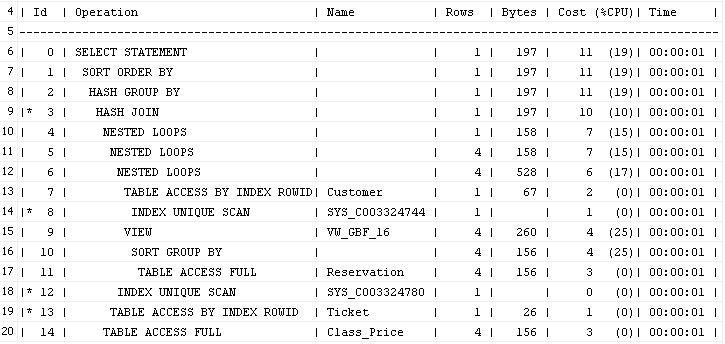
\includegraphics[scale=0.85]{pred_opt.png}
        \caption{Před optimalizací}
    \end{figure}
    \begin{figure}
        \centering
        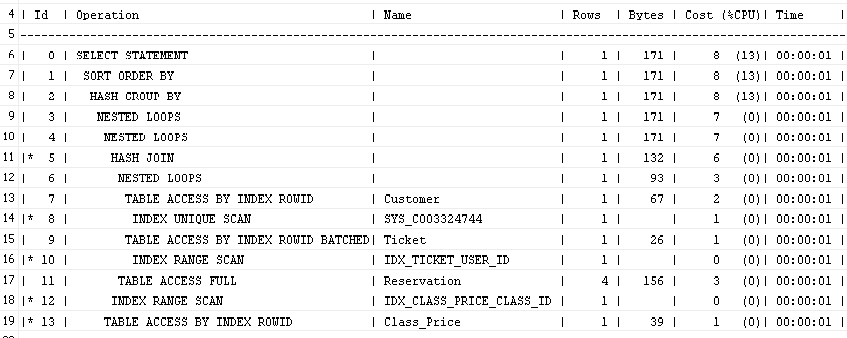
\includegraphics[scale=0.85]{po_opt.png}
        \caption{Po optimalizací}
    \end{figure}
\end{document}
